\documentclass[tikz,border=10pt]{standalone}
% Shared look for every TikZ diagram. Load with \input{../../tools/tikz-style.tex}
\usepackage[T1]{fontenc}
\usepackage{lmodern}
\renewcommand{\sfdefault}{lmr}  % diagrams use the same serif as the text
\usetikzlibrary{arrows.meta, positioning, shapes.geometric, calc, fit, backgrounds}
\definecolor{cblue}{HTML}{4C78A8}
\definecolor{corange}{HTML}{F58518}
\definecolor{cgreen}{HTML}{54A24B}
\definecolor{cred}{HTML}{E45756}
\definecolor{cpurple}{HTML}{B279A2}
\definecolor{cgrey}{HTML}{6B6B6B}
\tikzset{
  every picture/.style={font=\sffamily, line width=1.2pt},
  box/.style={draw=#1, fill=#1!12, rounded corners=4pt, align=center, inner sep=7pt, minimum height=1.1cm},
  box/.default=cgrey,
  arrow/.style={-{Stealth[length=3mm]}, draw=cgrey, line width=1.4pt},
  title/.style={font=\sffamily\bfseries\Large},
  note/.style={font=\sffamily\small, text=cgrey, align=center},
}
\AtBeginDocument{\hyphenpenalty=10000 \exhyphenpenalty=10000}

\begin{document}
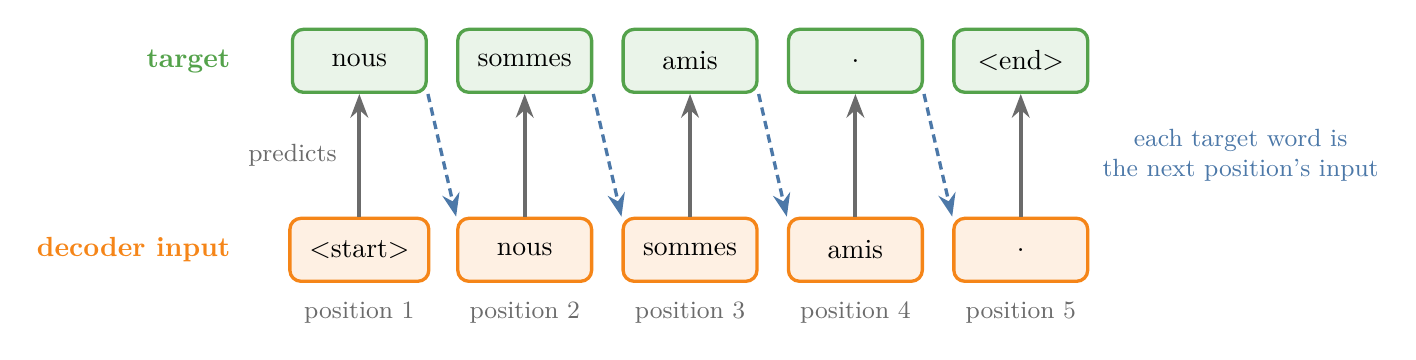
\begin{tikzpicture}[i/.style={box=corange, minimum width=1.7cm, minimum height=0.8cm, font=\sffamily},
  t/.style={box=cgreen, minimum width=1.7cm, minimum height=0.8cm, font=\sffamily}]
  \node[anchor=east, font=\sffamily\bfseries, text=cgreen] at (0.6,2.4) {target};
  \node[anchor=east, font=\sffamily\bfseries, text=corange] at (0.6,0) {decoder input};
  \foreach \a/\b [count=\k] in {{\textless start\textgreater}/nous, nous/sommes, sommes/amis, amis/., ./{\textless end\textgreater}} {
    \node[i] (i\k) at (2.1*\k,0) {\a};
    \node[t] (t\k) at (2.1*\k,2.4) {\b};
    \draw[arrow] (i\k) -- (t\k);
    \node[note] at (2.1*\k,-0.8) {position \k};
  }
  \foreach \k [evaluate=\k as \n using int(\k+1)] in {1,2,3,4} \draw[cblue, densely dashed, -{Stealth}, line width=1.2pt] (t\k.south east) -- (i\n.north west);
  \node[note, anchor=east] at (1.95,1.2) {predicts};
  \node[note, text=cblue, anchor=west] at (11.4,1.2) {each target word is\\the next position's input};
\end{tikzpicture}
\end{document}
